\documentclass[12pt]{beamer}
\usepackage{Estilos/BeamerFC}
\usepackage{Estilos/ColoresLatex}
\usetheme{Warsaw}
\usecolortheme{seahorse}
%\useoutertheme{default}
\setbeamercovered{invisible}
% or whatever (possibly just delete it)
\setbeamertemplate{section in toc}[sections numbered]
\setbeamertemplate{subsection in toc}[subsections numbered]
\setbeamertemplate{subsection in toc}{\leavevmode\leftskip=3.2em\rlap{\hskip-2em\inserttocsectionnumber.\inserttocsubsectionnumber}\inserttocsubsection\par}
\setbeamercolor{section in toc}{fg=blue}
\setbeamercolor{subsection in toc}{fg=blue}
\setbeamercolor{frametitle}{fg=blue}
\setbeamertemplate{caption}[numbered]

\setbeamertemplate{footline}
\beamertemplatenavigationsymbolsempty
\setbeamertemplate{headline}{}


\makeatletter
\setbeamercolor{section in foot}{bg=gray!30, fg=black!90!orange}
\setbeamercolor{subsection in foot}{bg=blue!30}
\setbeamercolor{date in foot}{bg=black}
\setbeamertemplate{footline}
{
  \leavevmode%
  \hbox{%
  \begin{beamercolorbox}[wd=.333333\paperwidth,ht=2.25ex,dp=1ex,center]{section in foot}%
    \usebeamerfont{section in foot} \insertsection
  \end{beamercolorbox}%
  \begin{beamercolorbox}[wd=.333333\paperwidth,ht=2.25ex,dp=1ex,center]{subsection in foot}%
    \usebeamerfont{subsection in foot}  \insertsubsection
  \end{beamercolorbox}%
  \begin{beamercolorbox}[wd=.333333\paperwidth,ht=2.25ex,dp=1ex,right]{date in head/foot}%
    \usebeamerfont{date in head/foot} {T1 - Segunda presentación} \hspace*{2em}
    \insertframenumber{} / \inserttotalframenumber \hspace*{2ex} 
  \end{beamercolorbox}}%
  \vskip0pt%
}
\makeatother

\makeatletter
\patchcmd{\beamer@sectionintoc}{\vskip1.5em}{\vskip0.8em}{}{}
\makeatother
\usepackage{pifont}
\newcommand{\cmark}{\ding{51}}%
\newcommand{\xmark}{\ding{55}}%

\makeatletter
\setbeamertemplate{footline}
{
  \leavevmode%
  \hbox{%
  \begin{beamercolorbox}[wd=.333333\paperwidth,ht=2.25ex,dp=1ex,center]{section in foot}%
    \usebeamerfont{section in foot} \insertsection
  \end{beamercolorbox}%
  \begin{beamercolorbox}[wd=.333333\paperwidth,ht=2.25ex,dp=1ex,center]{subsection in foot}%
    \usebeamerfont{subsection in foot}  \insertsubsection
  \end{beamercolorbox}%
  \begin{beamercolorbox}[wd=.333333\paperwidth,ht=2.25ex,dp=1ex,right]{date in head/foot}%
    \usebeamerfont{date in head/foot} \insertshortdate{} \hspace*{2em}
    \insertframenumber{} / \inserttotalframenumber \hspace*{2ex} 
  \end{beamercolorbox}}%
  \vskip0pt%
}
\makeatother

\sisetup{
  per-mode=fraction,
  fraction-function=\tfrac
}

\setbeamertemplate{navigation symbols}{}
\date{20 de abril}

% \sisetup{math-rm=\symup,detect-all}
\sisetup{detect-all, math-rm = \ensuremath}

\title{Sesión 8. Física}
\subtitle{Asesoría}

\begin{document}

\maketitle
\fontsize{14}{14}\selectfont
\spanishdecimal{.}

\section*{Contenido}
\frame[allowframebreaks]{\tableofcontents[currentsection, hideallsubsections]}

\subsection{Ejercicios - Guía}

\begin{frame}
\frametitle{Lo que hay que obtener}
Para cada problema determina:
\pause
\setbeamercolor{item projected}{bg=ao,fg=bananayellow}
\setbeamertemplate{enumerate items}{%
\usebeamercolor[bg]{item projected}%
\raisebox{1.5pt}{\colorbox{bg}{\color{fg}\footnotesize\insertenumlabel}}%
}
\begin{enumerate}[<+->]
\item El diagrama de cuerpo libre.
\item Las tensiones que se indican en cada problema.
\end{enumerate}
\end{frame}

\subsection*{Ejercicio 6}

\begin{frame}
\frametitle{Enunciado del Ejercicio 6}
Dos cuerdas se extienden entre dos postes. Una persona de \SI{65}{\kilo\gram} cuelga de ellas como se muestra en la siguiente figura.
\\
\bigskip
\pause
Encuentra la tensión en cada una de las cuerdas.
\end{frame}
\begin{frame}
\frametitle{Figura del Ejercicio 6}
\begin{figure}
  \centering
  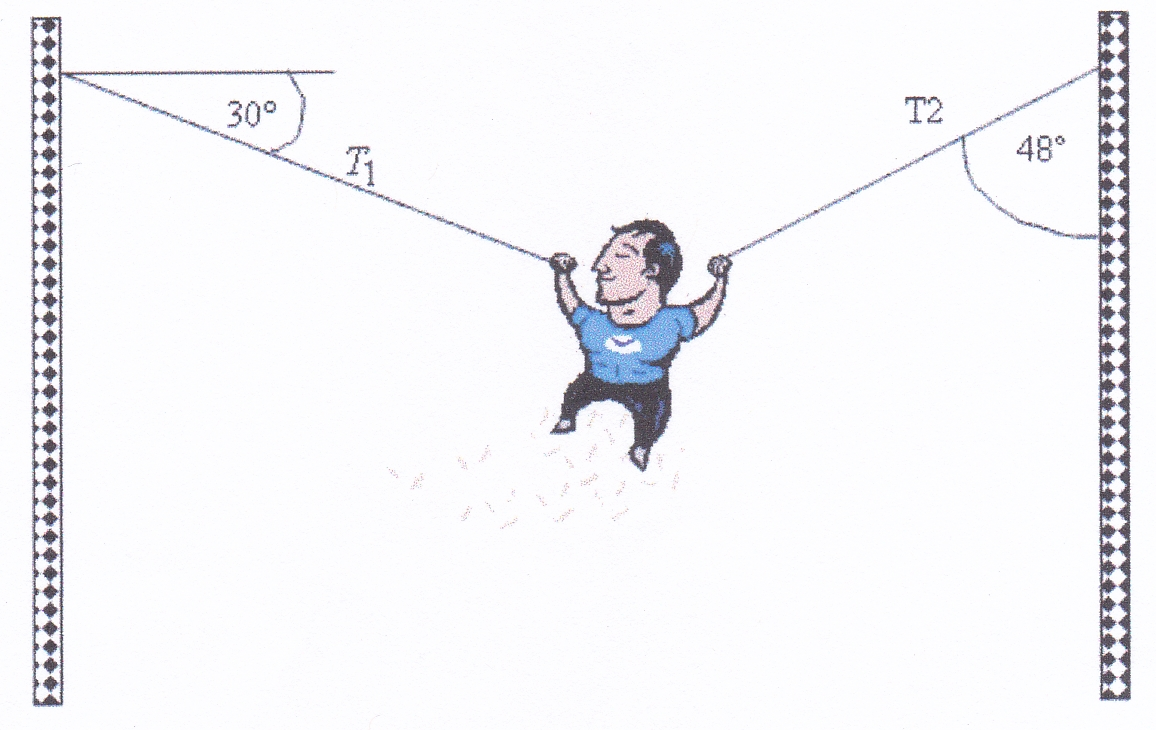
\includegraphics[scale=1]{Imagenes/DCL_Problema_06.png}
\end{figure}
\end{frame}
\begin{frame}
\frametitle{Revisando el enunciado}
Tomemos en cuenta que el ejercicio nos indica que la persona tiene una masa de \SI{65}{\kilo\gram}, por lo que la fuerza debida a la aceleración de la gravedad es:
\pause
\begin{eqnarray*}
\begin{aligned}
F &= - m \, g = \pause - \SI{65}{\kilogram} \cdot \SI{9.81}{\meter\per\square\second} = \\[0.5em] \pause
&= - \SI{637.65}{\newton}
\end{aligned}
\end{eqnarray*}
\pause
Esta fuerza la representamos con un vector cuya dirección está en el eje $y$ negativo.
\end{frame}
\begin{frame}
\frametitle{Diagrama de cuerpo libre}
\begin{figure}
\centering
\begin{tikzpicture}[scale=0.7]
  
  \draw (-5, 0) -- (5, 0);
  \draw [-stealth, thick, color=ao] (0, 0) -- (0, -6.37) node [right, midway] {\small{$-m \, g$}};

  \pause
  \draw (-4.31, 2.94) -- (-3, 2.94);
  \draw [color=red] (-3.81, 2.94) arc (0:-30:0.5);
  \node at (-3, 2.5) [color=red] {\small{$\theta_{1}$}};
  \draw [-stealth, thick, color=red] (0, 0) -- (-4.31, 2.94) node [above, midway] {\small{$T_{1}$}};
  \node at (-5.5, 2.3) {\small{$\theta_{1} = \ang{30}$}};

  \pause
  \draw [color=red] (-0.5, 0) arc(180:150:0.5);
  \node at (-1.5, 0.4) [color=red] {\small{$\theta_{1}$}};

  \pause
  \draw (4.31, 3.88) -- (4.31, 2.5);
  \draw (4.31, 3.4) arc(270:222:0.5);
  \node at (3.9, 3) {\small{$\alpha$}};
  \node at (5.7, 3.3) {\small{$\alpha = \ang{48}$}};
  \draw [-stealth, thick, color=red] (0, 0) -- (4.31, 3.88) node [above, midway] {\small{$T_{2}$}};
  \pause
  \node at (5.7, 2.6) {\small{$\theta_{2} = \ang{42}$}};
  \draw (4.31, 3.88) -- (3, 3.88);
  \draw [color=red] (3.81, 3.88) arc (180:222:0.5);
  \node at (3, 3.35) [color=red] {\small{$\theta_{2}$}};

  \draw [color=red] (0.5, 0) arc(0:42:0.5);
  \node at (1.5, 0.4) [color=red] {\small{$\theta_{2}$}};

  \pause
  \node at (6.3, 1.9) {\small{$\alpha + \theta_{2} = \ang{90}$}};
\end{tikzpicture}
\end{figure}
\end{frame}
\begin{frame}
\frametitle{Organizando la información}
Como en el caso de los sistemas de unidades, nos cviene organizar los vectores para ocuparlos posteriormente:
\pause
\begin{table}
\centering
\begin{tabular}{c | c | c}
Vector & Magnitud & Ángulo \\ \hline
$F = - m\, g$ & \SI{637.65}{\newton} & \ang{270} \\ \hline
$T_{1}$ & $T_{1}$ & $\theta_{1} = \ang{30}$ \\ \hline
$T_{2}$ & $T_{2}$ & $\theta_{2} = \ang{42}$ \\ \hline
\end{tabular}
\end{table}
\end{frame}
\begin{frame}
\frametitle{Descomposición de los vectores}
Ahora procedemos a obtener las componentes tanto en $x$ como en $y$ de cada vector enlistado en la diapositiva anterior.
\end{frame}
\begin{frame}
\frametitle{Descomposición de los vectores}
\begin{table}
\centering
\begin{tabular}{c | c | c }
Componente & Expresión & Sustitución \\ \hline
$F_{x}$ & $(\cos \ang{270})(\SI{637.65}{\newton})$ & $(0)(\SI{637.65}{\newton})$ \\ \hline
$F_{y}$ & $(\sin \ang{270})(\SI{637.65}{\newton})$ & $(-1)(\SI{637.65}{\newton})$ \\ \hline
\end{tabular}
\end{table}
Tenemos que:
\begin{align*}
F_{x} &= 0 \\
F_{y} &=  -\SI{637.65}{\newton}
\end{align*}
\end{frame}
\begin{frame}
\frametitle{Descomposición de los vectores}
\begin{table}
\centering
\begin{tabular}{c | c | c }
Componente & Expresión & Sustitución \\ \hline    
$T_{1x}$ & $\cos(\ang{30})(T_{1})$ & $(0.866)(T_{1})$ \\ \hline
$T_{2y}$ & $\sin(\ang{30})(T_{1})$ & $(0.5)(T_{1})$ \\ \hline
$T_{2x}$ & $\cos(\ang{42})(T_{2})$ & $(0.743)(T_{2})$ \\ \hline
$T_{2y}$ & $\sin(\ang{42})(T_{2})$ & $(0.669)(T_{2})$ \\ \hline
\end{tabular}
\end{table}
\end{frame}
\begin{frame}
\frametitle{Condiciones de equilibrio}
Sabemos que si el sistema está en equilibrio, la suma de las componentes de las fuerzas tano en la dirección $x$, como en $y$ valen cero:
\pause
\begin{eqnarray*}
\begin{aligned}
\nsum F_{x} &= 0 \\[0.5em] \pause 
\nsum F_{y} &= 0
\end{aligned}
\end{eqnarray*}
\end{frame}
\begin{frame}
\frametitle{Condiciones de equilibrio}
Tendremos entonces las componentes en $x$ son:
\begin{eqnarray*}
\begin{aligned}
\nsum F_{x} &= T_{1x} + T_{2x} + F_{x} = 0 \\[0.5em] \pause
\nsum F_{x} &= -\cos \ang{30} \cdot T_{1} + \cos \ang{42} \cdot T_{2} + 0 = 0 \\[0.5em] \pause
\nsum F_{x} &= -0.866 \cdot T_{1} + 0.7431 \cdot T_{2} = 0 
\end{aligned}
\end{eqnarray*}
\end{frame}
\begin{frame}
\frametitle{Condiciones de equilibrio}
Las componentes en $y$ son:
\begin{eqnarray*}
\begin{aligned}
\nsum F_{y} &= T_{1y} + T_{2y} + F_{y} = 0 \\[0.5em] \pause
\nsum F_{y} &= \sen \ang{30} \cdot T_{1} + \sin \ang{42} \cdot T_{2} - m \, g = 0 \\[0.5em] \pause
\nsum F_{y} &= 0.5 \cdot T_{1} + 0.6691 \cdot T_{2} - \SI{637.65}{\newton} = 0 \\[0.5em] \pause
\end{aligned}
\end{eqnarray*}
\end{frame}
\begin{frame}
\frametitle{Sistema de dos ecuaciones}
Con las expresiones anteriores se obtiene un sistema de dos ecuaciones simultáneas con dos incógnitas:
\pause
\begin{align*}
-0.866 \cdot T_{1} + 0.7431 \cdot T_{2} &= 0 \\[0.5em]
0.5 \cdot T_{1} + 0.6691 \cdot T_{2} - \SI{637.65}{\newton} &= 0
\end{align*}
\pause
De donde podemos utilizar cualquier técnica para resolver este sistema simultáneo de dos ecuaciones.
\end{frame}
\begin{frame}
\frametitle{Resolviendo el sistema de ecuaciones}
Acomodando los términos del sistema, se tiene:
\pause
\begin{align}
-0.866 \cdot T_{1} + 0.7431 \cdot T_{2} &= 0 \label{eq:ecuacion_01} \\[0.5em]
0.5 \cdot T_{1} + 0.6691 \cdot T_{2} &= \SI{637.65}{\newton} \label{eq:ecuacion_02}
\end{align}
\pause
De la ecuación (\ref{eq:ecuacion_01}) despejamos el valor de $T_{2}$:
\pause
\begin{eqnarray*}
\begin{aligned}
0.7431 \cdot T_{2} &= 0.866 \cdot T_{1} \\ \pause
T_{2} = \dfrac{0.866}{0.7431} \cdot T_{1} &= \pause 1.1653 \cdot T_{1}
\end{aligned}
\end{eqnarray*}
\end{frame}
\begin{frame}
\frametitle{Resolviendo las tensiones}
El valor anterior de $T_{2}$ lo sustituimos en la ecuación (\ref{eq:ecuacion_02}), para obtener $T_{1}$:
\pause
\begin{eqnarray*}
\begin{aligned}
0.5 \cdot T_{1} + 0.6691 \cdot (1.1653 \, T_{1}) &= \SI{637.65}{\newton} \\[0.5em] \pause
0.5 \cdot T_{1} + 0.7797 \cdot T_{1} &= \SI{637.65}{\newton} \\[0.5em] \pause
1.2797 \cdot T_{1} &= \SI{637.65}{\newton} \\[0.5em] \pause
T_{1} &= \dfrac{\SI{637.65}{\newton}}{1.2797} = \pause \SI{498.28}{\newton}
\end{aligned}
\label{eq:ecuacion_03}
\end{eqnarray*}
\end{frame}
\begin{frame}
\frametitle{Obteniendo el segundo término}
Una vez obtenido $T_{1}$ usamos este valor para calcular $T_{2}$, para ello ocupamos la ecuación (\ref{eq:ecuacion_01})
\pause
\begin{eqnarray*}
\begin{aligned}
-0.866 \cdot T_{1} + 0.7431 \cdot T_{2} &= 0 \\[0.5em] \pause
-0.866 \cdot \SI{498.28}{\newton} + 0.7431 \cdot T_{2} &= 0
\end{aligned}
\end{eqnarray*}
\end{frame}
\begin{frame}
\frametitle{Obteniendo el segundo término}
Reacomodamos los términos:
\pause
\begin{eqnarray*}
\begin{aligned}
0.7431 \cdot T_{2} &= 0.866 \cdot \SI{498.28}{\newton} \\[0.5em] \pause
T_{2} &= \dfrac{0.866}{0.7431} \cdot \SI{498.28}{\newton} \\[0.5em] \pause
T_{2} &= 1.1653 \cdot \SI{498.28}{\newton} \\[0.5em] \pause
T_{2} &= \SI{580.68}{\newton}
\end{aligned}
\end{eqnarray*}
\end{frame}
\begin{frame}
\frametitle{Ejercicio resuelto}
De esta manera hemos obtenido las tensiones en las cuerdas, que es lo que nos pide el ejercicio:
\begin{align*}
T_{1} &= \SI{498.28}{\newton} \\[0.5em]
T_{2} &= \SI{580.68}{\newton}
\end{align*}
\end{frame}

\subsection*{Ejercicio 7}

\begin{frame}
\frametitle{Enunciado del Ejercicio 7}
El hombre araña tiene una masa de \SI{72}{\kilo\gram} y está cargando a una mujer de \SI{60}{\kilo\gram}.
\\
\bigskip
\pause
¿Cuáles son las tensiones que se están ejerciendo en las \enquote{cuerdas} bajo la acción de estas masas?
\end{frame}
\begin{frame}
\frametitle{Figura del Ejercicio 7}
\begin{figure}
  \centering
  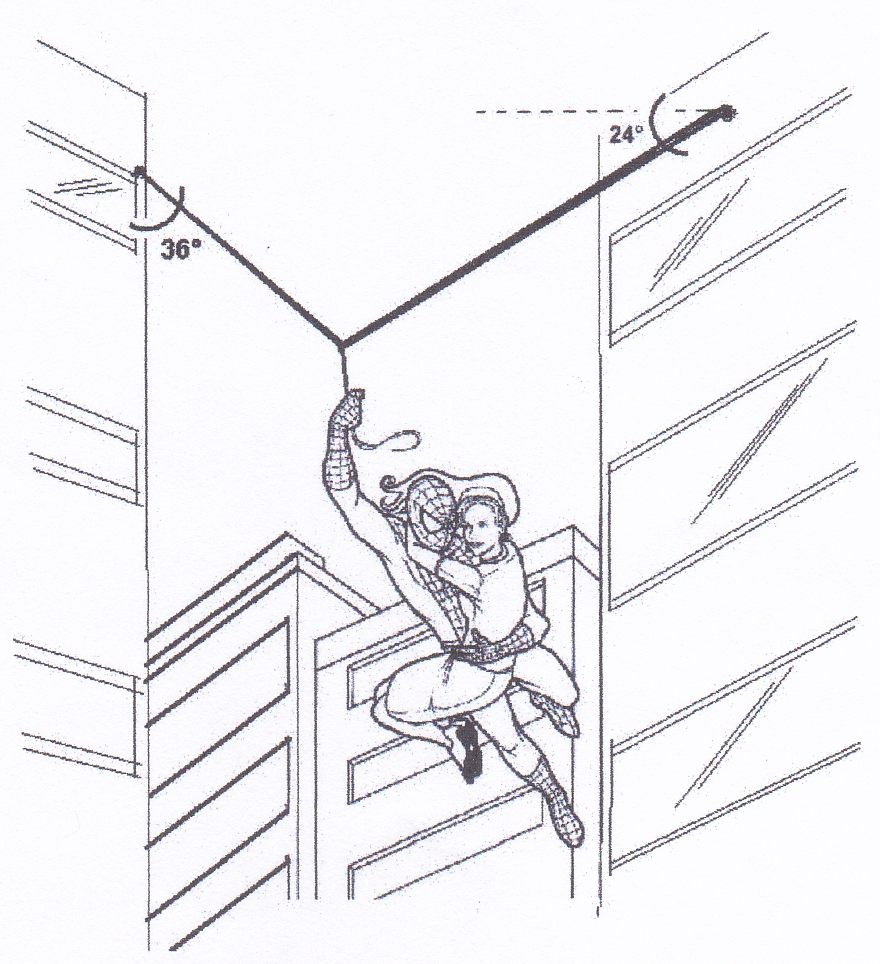
\includegraphics[scale=0.81]{Imagenes/DCL_Problema_07.png}
\end{figure}
\begin{tikzpicture}[overlay]
  \node at (4.2, 6) [color=ao] {\small{$T_{1}$}};
  \node at (6, 6.3) [color=ao] {\small{$T_{2}$}};
\end{tikzpicture}
\end{frame}

\end{document}